\documentclass[12pt]{article}
%% arXiv paper template by Flip Tanedo


%%%%%%%%%%%%%%%%%%%%%%%%%%%%%
%%%  THE USUAL PACKAGES  %%%%
%%%%%%%%%%%%%%%%%%%%%%%%%%%%%

\usepackage{amsmath}         % \
\usepackage{amssymb}         %  | AMS Packages for math
\usepackage{amsfonts}        % /
\usepackage{graphicx}        % Graphics
 

%%%%%%%%%%%%%%%%%%%%%%%%%%%%%%%%%
%%%  UNUSUAL PACKAGES        %%%%
%%%  Uncomment as necessary. %%%%
%%%%%%%%%%%%%%%%%%%%%%%%%%%%%%%%%

\usepackage{lipsum}        % block of text (formatting test)
%\usepackage{color}         % \color{...}, colored text
%\usepackage{slashed}       % \slashed{k}
%\usepackage{framed}        % boxed remarks
%\usepackage{subcaption}    % subfigures; subfig depreciated
%\usepackage{mathrsfs}      % Weinberg-esque letters
%\usepackage{paralist}      % compactitem
%\usepackage{multirow}      % multiple row elements in a table
%\usepackage{cite}          % grouping citations (incompatible with collref)
%\usepackage{booktabs}      % tables
%\usepackage{nicefrac}      % fractions in tables,
%\usepackage{youngtab}	    % Young Tableaux
%\usepackage{arydshln} 	    % dashed lines in arrays and tables
%\usepackage{appendix}      % subappendices
%\usepackage{pifont}        % check marks
%\usepackage{bbm}           % \mathbbm{1} incompatible with XeLaTeX 


%%%%%%%%%%%%%%%%%%%%%%%%%%%%%%%%%%%%%%%%%%%
%%%  FLIP'S CUSTOM PACKAGES            %%%%
%%%  These are in separate .sty files  %%%%
%%%%%%%%%%%%%%%%%%%%%%%%%%%%%%%%%%%%%%%%%%%

\usepackage{flip-acronyms} % HEP acronyms in small caps, e.g. \GeV
\usepackage{tikzfeynman}   % Flip's Feynman Diagrams


%%%%%%%%%%%%%%%%%%%%%%%%%%%%%%%%%%%%%%%%%%%%%%%
%%%  PAGE FORMATTING and (RE)NEW COMMANDS  %%%%
%%%%%%%%%%%%%%%%%%%%%%%%%%%%%%%%%%%%%%%%%%%%%%%


\usepackage[margin=2cm]{geometry}   % reasonable margins
\graphicspath{{figures/}}	        % set directory for figures
\numberwithin{equation}{section}    % set equation numbering
\renewcommand{\tilde}{\widetilde}   % tilde over characters
\renewcommand{\vec}[1]{\mathbf{#1}} % vectors are boldface


\newcommand{\dbar}{d\mkern-6mu\mathchar'26}    % for d/2pi
\newcommand{\ket}[1]{\left|#1\right\rangle}    % <#1|
\newcommand{\bra}[1]{\left\langle#1\right|}    % |#1>
\newcommand{\Xmark}{\text{\sffamily X}}        % cross out


% Commands for temporary comments
\newcommand{\comment}[2]{\textcolor{red}{[\textbf{#1} #2]}}
\newcommand{\flip}[1]{{\tt \color{red} [Flip: {#1}]}}
\newcommand{\email}[1]{\href{mailto:#1}{#1}}


\newenvironment{institutions}[1][2em]{\begin{list}{}{\setlength\leftmargin{#1}\setlength\rightmargin{#1}}\item[]}{\end{list}}


%%%%%%%%%%%%%%%%%%%%%%%%%%%%%%%%%%%%%%%%%%%%%%
%%%  TIKZ COMMANDS FOR EXTERNAL DIAGRAMS  %%%%
%%%  requires -shell-escape               %%%%
%%%%%%%%%%%%%%%%%%%%%%%%%%%%%%%%%%%%%%%%%%%%%%

%\usetikzlibrary{external}
%\tikzexternalize[prefix=tikz/] % folder for external pdfs



%%%%%%%%%%%%%%%%%%%
%%%  HYPERREF  %%%%
%%%%%%%%%%%%%%%%%%%

% This package has to be at the end; can lead to conflicts
\usepackage[
	colorlinks=true,
	citecolor=black,
	linkcolor=black,
	urlcolor=blue,
	hypertexnames=false]{hyperref}



%%%%%%%%%%%%%%%%%%%%%
%%%  TITLE DATA  %%%%
%%%%%%%%%%%%%%%%%%%%%


\begin{document}

\thispagestyle{empty}
\begin{center}

    {\huge \textbf{Sample Feynman Diagrams in TikZ} \\
    \large \textsc{Vol.~II: [non-Feynman] Diagrams} }

    \vskip .7cm

    { \bf Flip Tanedo } 
    \\ \vspace{-.2em}
    { \tt
    \footnotesize
    \email{flip.tanedo@uci.edu} 
    }
	
    \vspace{-.2cm}

    \begin{institutions}[2.25cm]
    \footnotesize
	\vspace*{0.05cm}
	{\it 
	    Department of Physics \& Astronomy, 
	    University of California, 
	    Irvine, \textsc{ca} 92697
	    }   
    \end{institutions}

\end{center}



%%%%%%%%%%%%%%%%%%%%%
%%%  ABSTRACT    %%%%
%%%%%%%%%%%%%%%%%%%%%

\begin{abstract}
\noindent This is collection of useful sample Feynman diagrams and pieces typeset in TikZ. See Volume I for background information.
\end{abstract}




%%%%%%%%%%%%%%%%%%%%%
%%%  THE MEAT    %%%%
%%%%%%%%%%%%%%%%%%%%%

% Use \input if you have separate files.
% \include is `smarter' (creates separate aux files for each tex file) 
% and hence more efficient, but it automatically puts a page break
% between included files. Input doesn't do this.



\section{Bezier graphs}

\begin{center}
	\begin{tikzpicture}[line width =1.5]
		\draw[fill=black] (0,0) circle (.075);
		\draw[fermion] (0,0) -- (2.5,0);
		\draw[fermionbar] (2.5,0) -- (4.5,0);
		\draw[dashed] (4.5,0) -- (5.5,0) node[right] {$g$};
		\draw[fill=black] (2.5,0) circle (.075);
		\node[below] at (2.5,0) {$g_*$};
		%
		\draw[fermion] (0,3) -- (0,0);
		\draw[dashed] (0,3) -- (0,3.5) node[above] {$y$};
		%
		% Bezier Curve!
		\draw[fermion, line width=1] (.3,3) .. controls (.7,.2) and (.75,.2) .. (3,2);
		\draw[fermion, line width=1] (0,0) to [out=15, in=240] (3,2);
		\draw[fermion, line width=1] (2.5,0) -- (3,2);
		\draw[fermion, line width=1] (4.5,.2) .. controls (3,.7) and (3.2,.4) .. (3,2);
		%
		\draw[fill=black] (3,2) circle (.075);
		\draw[fermion, line width=1] (.5,3) .. controls (1,1) and (1.2,1) .. (3,2);
		\draw[fermion, line width=1] (4.5,3) .. controls (3,2.5) and (3.5,2.5) .. (3,2);
		\draw[fermion, line width=1] (1.5,3) to [out = -20, in = 110] (3,2);
		\node[right] at (3,2) {$(\hat g, \hat y)$};
	\end{tikzpicture}	
\end{center}


\section{Seiberg duality }

\subsection{Deconstruction of XD}

	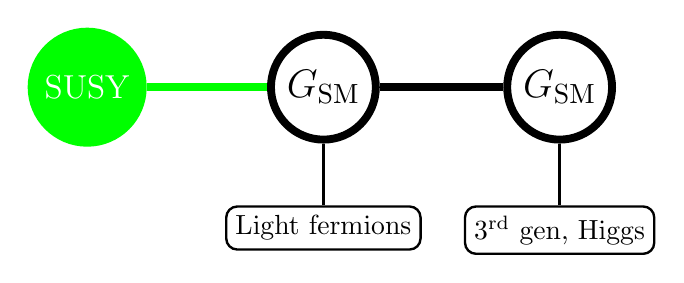
\begin{tikzpicture}%[show background grid] %% Use grid for positioning, then turn off
	 \node[circle, draw, line width=1mm, minimum size = 1.2cm] (GSM1) at (0,0) {\Large $G_\text{SM}$};
	 \node[circle, draw, line width=1mm, minimum size = 1.2cm, fill, color=green] (SUSY) at (-3,0) {\large \textcolor{white}{$\text{SUSY}$}};
	 \node[circle, draw, line width=1mm, minimum size = 1.2cm] (GSM2) at (3,0) {\Large $G_\text{SM}$};
	 \draw[color=green, line width=1mm] (SUSY) -- (GSM1);
	 \draw[line width=1mm] (GSM1) -- (GSM2);
	 %
	 \node[draw, anchor=north, rounded corners, line width=.2ex]
	 	(lightfermions) at (0,-1.5) {\normalsize Light fermions};
	  \node[draw, anchor=north, rounded corners, line width=.2ex] 
	  	(gen3) at (3,-1.5) {\normalsize 3$^\text{rd}$ gen, Higgs};
	  \draw[line width=.2ex] (lightfermions) -- (GSM1);
	  \draw[line width=.2ex] (gen3) -- (GSM2);
	\end{tikzpicture}
	
\subsection{Quiver for electric theory}

	\begin{tikzpicture}%[show background grid] %% Use grid for positioning, then turn off
	 \node[circle, draw, line width=1mm, minimum size = 1.2cm] (F1) at (-3,0) {\Large $F$};
	 \node[circle, draw, line width=1mm, minimum size = 1.2cm] (F2) at (3,0) {\Large $F$};
	 \node[circle, draw, line width=1mm, minimum size = 1.2cm, fill, color=green] (N) at (0,0) {\large \textcolor{white}{$N$}};
	 %
    \draw[fermion, line width=1mm] (F1) -- (N);
    \draw[fermion, line width=1mm] (N) -- (F2);
	\end{tikzpicture}
	
\subsection{Quiver for magnetic theory}
	
		\begin{tikzpicture}%[show background grid] %% Use grid for positioning, then turn off
	 \node[circle, draw, line width=1mm, minimum size = 1.2cm] (F1) at (-3,0) {\Large $F$};
	 \node[circle, draw, line width=1mm, minimum size = 1.2cm] (F2) at (3,0) {\Large $F$};
	 \node[circle, draw, line width=1mm, minimum size = 1.2cm, fill, color=green] (N) at (0,0) {\large \textcolor{white}{$F-N$}};
	 %
    \draw[fermion, line width=1mm] (F1) -- (N);
    \draw[fermion, line width=1mm] (N) -- (F2);
    \draw[fermion, line width=1mm] (F1) arc (180:0:3);
    \node[circle, draw, line width=1mm, minimum size = 1.2cm, fill=white] at (F1) {\Large $F$};
	 \node[circle, draw, line width=1mm, minimum size = 1.2cm, fill=white] at (F2) {\Large $F$};
	\end{tikzpicture}
	




\section{Phase structure of SQCD}

\begin{center}
	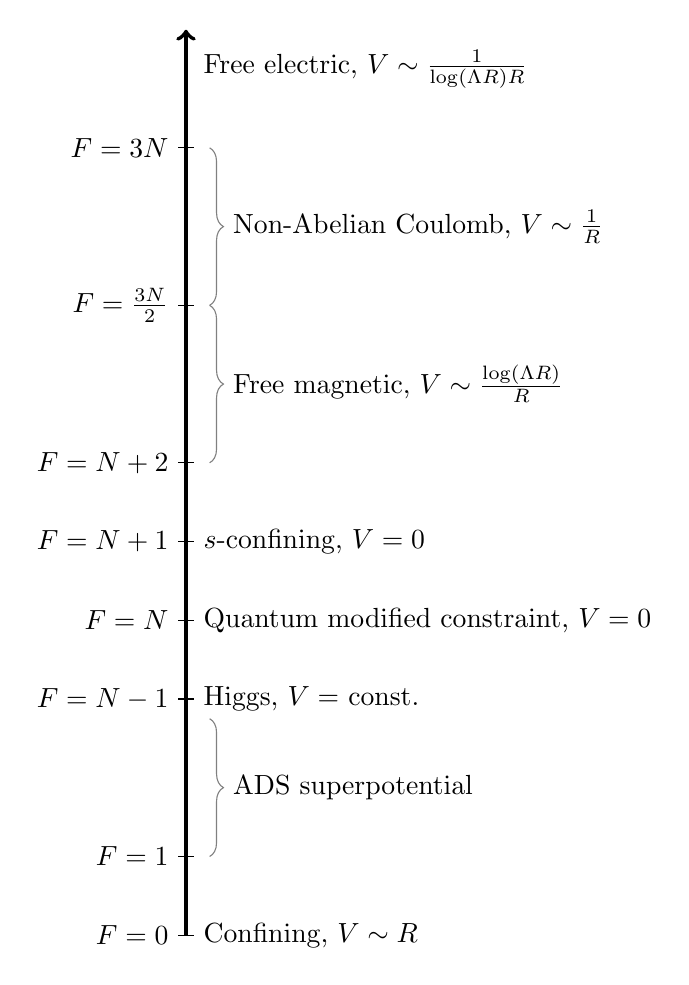
\begin{tikzpicture}
		\draw[->,line width=1.5] (0,0) -- (0,11.5);
		\draw (-.1,0) node[left] {$F=0$} -- (.1,0) node[right] {Confining, $V\sim R$};
		\draw (-.1,1) node[left] {$F=1$} -- (.1,1);
		\draw (-.1,3) node[left] {$F=N-1$} -- (.1,3) node[right] {Higgs, $V=$ const.};
		\draw [gray,decorate,decoration={brace,amplitude=5pt}]
		   (.3,2.75)  -- (.3,1) 
		   node [right,black,midway,xshift=5] {ADS superpotential};
		\draw (-.1,4) node[left] {$F=N$} -- (.1,4) node[right] {Quantum modified constraint, $V=0$};
		\draw (-.1,5) node[left] {$F=N+1$} -- (.1,5) node[right] {$s$-confining, $V=0$};
		\draw (-.1,6) node[left] {$F=N+2$} -- (.1,6);
		\draw (-.1,8) node[left] {$F=\frac {3N}2$} -- (.1,8);
		\draw [gray,decorate,decoration={brace,amplitude=5pt}]
		   (.3,8)  -- (.3,6) 
		   node [right,black,midway,xshift=5] {Free magnetic, $V\sim \frac{\log(\Lambda R)}R$};
		\draw (-.1,10) node[left] {$F=3N$} -- (.1,10);
		\draw [gray,decorate,decoration={brace,amplitude=5pt}]
		   (.3,10)  -- (.3,8) 
		   node [right,black,midway,xshift=5] {Non-Abelian Coulomb, $V\sim \frac 1R$};
		\node[right] at (.1,11) {Free electric, $V\sim \frac{1}{\log(\Lambda R)R}$};
	\end{tikzpicture}
\end{center}


\section{Dynkin diagrams}

From \texttt{http://doxdrum.wordpress.com/2012/04/02/latex-tip-dynkin-diagrams-using-tikz/}

\begin{center}
  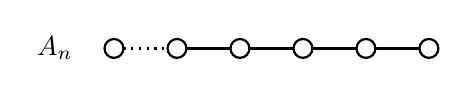
\begin{tikzpicture}[scale=.4]
    \draw (-1,0) node[anchor=east]  {$A_n$};
    \foreach \x in {0,...,5}
    \draw[xshift=\x cm,thick] (\x cm,0) circle (.3cm);
    \draw[dotted,thick] (0.3 cm,0) -- +(1.4 cm,0);
    \foreach \y in {1.15,...,4.15}
    \draw[xshift=\y cm,thick] (\y cm,0) -- +(1.4 cm,0);
  \end{tikzpicture}
\end{center}

\begin{center}
  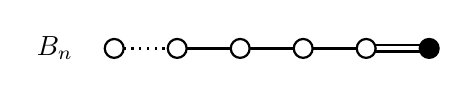
\begin{tikzpicture}[scale=.4]
    \draw (-1,0) node[anchor=east]  {$B_n$};
    \foreach \x in {0,...,4}
    \draw[xshift=\x cm,thick] (\x cm,0) circle (.3cm);
    \draw[xshift=5 cm,thick,fill=black] (5 cm, 0) circle (.3 cm);
    \draw[dotted,thick] (0.3 cm,0) -- +(1.4 cm,0);
    \foreach \y in {1.15,...,3.15}
    \draw[xshift=\y cm,thick] (\y cm,0) -- +(1.4 cm,0);
    \draw[thick] (8.3 cm, .1 cm) -- +(1.4 cm,0);
    \draw[thick] (8.3 cm, -.1 cm) -- +(1.4 cm,0);
  \end{tikzpicture}
\end{center}

\begin{center}
  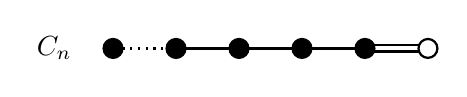
\begin{tikzpicture}[scale=.4]
    \draw (-1,0) node[anchor=east]  {$C_n$};
    \foreach \x in {0,...,4}
    \draw[xshift=\x cm,thick,fill=black] (\x cm,0) circle (.3cm);
    \draw[xshift=5 cm,thick] (5 cm, 0) circle (.3 cm);
    \draw[dotted,thick] (0.3 cm,0) -- +(1.4 cm,0);
    \foreach \y in {1.15,...,3.15}
    \draw[xshift=\y cm,thick] (\y cm,0) -- +(1.4 cm,0);
    \draw[thick] (8.3 cm, .1 cm) -- +(1.4 cm,0);
    \draw[thick] (8.3 cm, -.1 cm) -- +(1.4 cm,0);
  \end{tikzpicture}
\end{center}

\begin{center}
  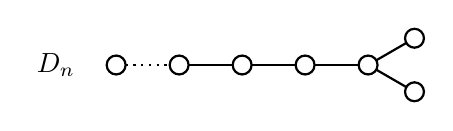
\begin{tikzpicture}[scale=.4]
    \draw (-1,0) node[anchor=east]  {$D_n$};
    \foreach \x in {0,...,4}
    \draw[xshift=\x cm,thick] (\x cm,0) circle (.3cm);
    \draw[xshift=8 cm,thick] (30: 17 mm) circle (.3cm);
    \draw[xshift=8 cm,thick] (-30: 17 mm) circle (.3cm);
    \draw[dotted,thick] (0.3 cm,0) -- +(1.4 cm,0);
    \foreach \y in {1.15,...,3.15}
    \draw[xshift=\y cm,thick] (\y cm,0) -- +(1.4 cm,0);
    \draw[xshift=8 cm,thick] (30: 3 mm) -- (30: 14 mm);
    \draw[xshift=8 cm,thick] (-30: 3 mm) -- (-30: 14 mm);
  \end{tikzpicture}
\end{center}

\begin{center}
  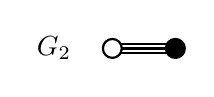
\begin{tikzpicture}[scale=.4]
    \draw (-1,0) node[anchor=east]  {$G_2$};
    \draw[thick] (0 ,0) circle (.3 cm);
    \draw[thick,fill=black] (2 cm,0) circle (.3 cm);
    \draw[thick] (30: 3mm) -- +(1.5 cm, 0);
    \draw[thick] (0: 3 mm) -- +(1.4 cm, 0);
    \draw[thick] (-30: 3 mm) -- +(1.5 cm, 0);
  \end{tikzpicture}
\end{center}

\begin{center}
  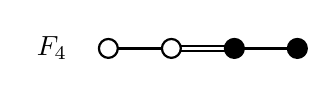
\begin{tikzpicture}[scale=.4]
    \draw (-3,0) node[anchor=east]  {$F_4$};
    \draw[thick] (-2 cm ,0) circle (.3 cm);
    \draw[thick] (0 ,0) circle (.3 cm);
    \draw[thick,fill=black] (2 cm,0) circle (.3 cm);
    \draw[thick,fill=black] (4 cm,0) circle (.3 cm);
    \draw[thick] (15: 3mm) -- +(1.5 cm, 0);
    \draw[xshift=-2 cm,thick] (0: 3 mm) -- +(1.4 cm, 0);
    \draw[thick] (-15: 3 mm) -- +(1.5 cm, 0);
    \draw[xshift=2 cm,thick] (0: 3 mm) -- +(1.4 cm, 0);
  \end{tikzpicture}
\end{center}

\begin{center}
  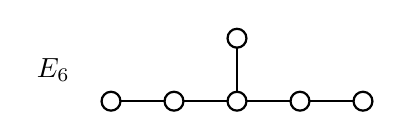
\begin{tikzpicture}[scale=.4]
    \draw (-1,1) node[anchor=east]  {$E_6$};
    \foreach \x in {0,...,4}
    \draw[thick,xshift=\x cm] (\x cm,0) circle (3 mm);
    \foreach \y in {0,...,3}
    \draw[thick,xshift=\y cm] (\y cm,0) ++(.3 cm, 0) -- +(14 mm,0);
    \draw[thick] (4 cm,2 cm) circle (3 mm);
    \draw[thick] (4 cm, 3mm) -- +(0, 1.4 cm);
  \end{tikzpicture}
\end{center}

\begin{center}
  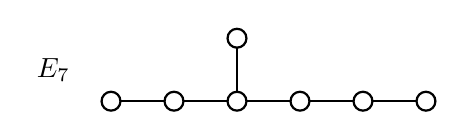
\begin{tikzpicture}[scale=.4]
    \draw (-1,1) node[anchor=east]  {$E_7$};
    \foreach \x in {0,...,5}
    \draw[thick,xshift=\x cm] (\x cm,0) circle (3 mm);
    \foreach \y in {0,...,4}
    \draw[thick,xshift=\y cm] (\y cm,0) ++(.3 cm, 0) -- +(14 mm,0);
    \draw[thick] (4 cm,2 cm) circle (3 mm);
    \draw[thick] (4 cm, 3mm) -- +(0, 1.4 cm);
  \end{tikzpicture}
\end{center}

\begin{center}
  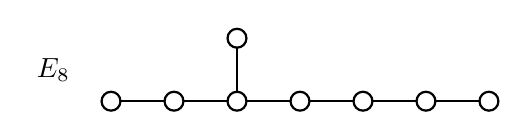
\begin{tikzpicture}[scale=.4]
    \draw (-1,1) node[anchor=east]  {$E_8$};
    \foreach \x in {0,...,6}
    \draw[thick,xshift=\x cm] (\x cm,0) circle (3 mm);
    \foreach \y in {0,...,5}
    \draw[thick,xshift=\y cm] (\y cm,0) ++(.3 cm, 0) -- +(14 mm,0);
    \draw[thick] (4 cm,2 cm) circle (3 mm);
    \draw[thick] (4 cm, 3mm) -- +(0, 1.4 cm);
  \end{tikzpicture}
\end{center}


\section{Composite Higgs}

%\begin{figure}
\begin{center}
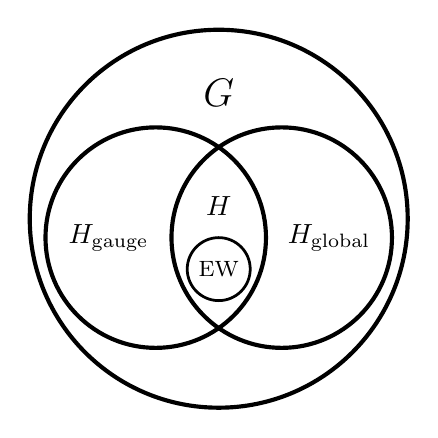
\begin{tikzpicture}[line width=1.5 pt, scale=.8]
\draw (0,0) circle (3);
\draw (1,-.3) circle (1.75);
\draw (-1,-.3) circle (1.75);
\node at (0,2) {\Large $G$};
\node at (1.75,-.3) { $H_\text{global}$};
\node at (-1.75,-.3) { $H_\text{gauge}$};
%\node at (0,-.3) {\Large $H$};
\node at (0,.2) {$H$};
\draw[line width=1pt] (0,-.8) circle (.5);
\node at (0,-.8) {\footnotesize EW};
\end{tikzpicture}
\qquad
\qquad
\qquad
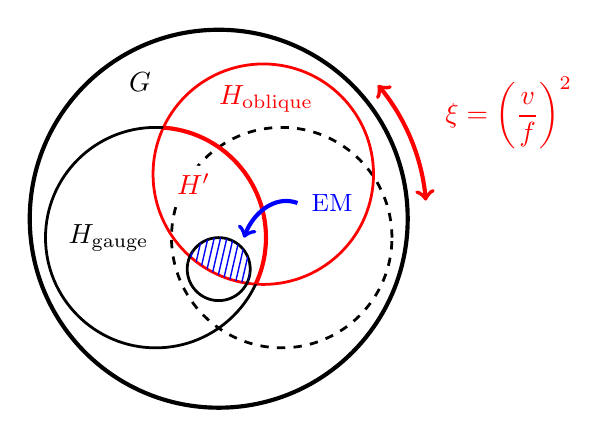
\begin{tikzpicture}[line width=1.5 pt, scale=.8]
\draw (0,0) circle (3);
\draw[line width=1pt, dashed] (1,-.3) circle (1.75);
\draw[line width=1pt, red] (45:1) circle (1.75);
\draw[line width=1pt] (-1,-.3) circle (1.75);
\draw[line width=1pt] (0,-.8) circle (.5);
%\node at (0,-.8) {EW};
%\node[scale=.75, rotate=-30] at (.09,-.65) {\footnotesize \textcolor{blue}{EM}};
\begin{scope}
	\clip (45:1) circle (1.75);
	\draw[line width=1.5pt, color=red] (-1,-.3) circle (1.75);
	\clip (0,-.8) circle (.5);
%	\draw[line width=1pt, fill=blue] (0,-.8) circle (.5);
	\foreach \x in {-1.9,-1.8,...,1.3}
	\draw[line width=.5 pt, color=blue] (\x,-1.3) -- (\x+.6,1.3);
\end{scope}
%\node[scale=.75, rotate=-30] at (.09,-.65) {\footnotesize \textcolor{white}{EM}};
%
\path[->, color=blue, line width=1.5] (1.25,.25) edge [out = 160, in = 70] (.4,-.3);
\node at (1.8,.25) {\small \textcolor{blue}{EM}};
%
\node at (120:2.5) {$G$};
%\node at (1.75,-.3) { $H_\text{global}$};
\node at (-1.75,-.3) { $H_\text{gauge}$};
\node at (.75,1.9) {\textcolor{red}{$H_\text{oblique}$}};
%\node at (0,.2) {$H$};
\fill[fill=white] (-.4,.5) circle (.35);
\node at (-.4,.55) {\textcolor{red}{$H'$}};
\draw[<->, color = red] (5:3.3) arc (5:40:3.3);
\node at (20:4.9) {\textcolor{red}{$\displaystyle \xi = \left(\frac{v}{f}\right)^2$}};
\end{tikzpicture}
\end{center}
%\caption{Pattern of symmetry breaking. (\textsc{left}) Strong dynamics breaks $G\to H_\text{global}$ spontaneously, while $H_\text{gauge} \subset G$ is explicitly broken through gauging. The unbroken group $H = H_\text{gauge}\cap H_\text{global}$ contains the \SM electroweak group, $\text{SU}(2)_\text{L}\times\text{U}(1)_\text{Y}$. (\textsc{right}) Vacuum misalignment from \SM interactions shifts the unbroken group $H\to H'$ and breaks the electroweak group to $\text{U}(1)_\text{EM}$. The degree of misalignment is parametrized by $\xi$, the squared ratio of the \EWSB \vev to the $G\to H$ \vev. Adapted from 
%\cite{SafariThesis}}
%\label{fig:comp:breaking:pattern}
%\end{figure}
%

\section{Collective Symmetry Breaking}

This is actually totally wrong... correct figure below.

\vspace{1em}

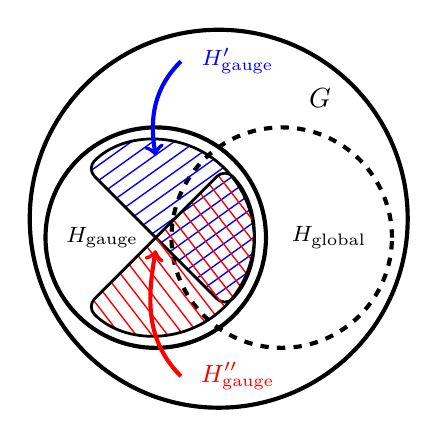
\begin{tikzpicture}[line width=1.5 pt, scale=.8]
\draw (0,0) circle (3);
\draw[dashed] (1,-.3) circle (1.75);
\draw (-1,-.3) circle (1.75);
\begin{scope}[shift={(-1.,-.3)}]
\begin{scope}[rotate=-45]
    \begin{scope}
    	\clip [rounded corners] (1.55,0) arc (0:180:1.55) -- cycle;
    	\foreach \x in {-1.9,-1.7,...,1.3}
	    \draw[line width=.5 pt, color=blue] (\x,-1.3) -- (\x+.6,2.3);
    \end{scope}
    \draw[rounded corners, line width=1] (1.55,0) arc (0:180:1.55) -- cycle;
\end{scope}
\begin{scope}[rotate=45]
    \begin{scope}
    	\clip [rounded corners] (-1.55,0) arc (180:360:1.55) -- cycle;
    	\foreach \x in {-1.9,-1.7,...,1.3}
	    \draw[line width=.5 pt, color=red] (\x,-2.3) -- (\x+.6,2.3);
    \end{scope}
    \draw[rounded corners, line width=1] (-1.55,0) arc (180:360:1.55) -- cycle;
\end{scope}
\end{scope}
%\draw[line width=2pt] (0,-.4) circle (.4);
\node at (1.75,-.3) {\footnotesize $H_\text{global}$};
\node at (-1.85,-.3) {\footnotesize $H_\text{gauge}$};
\node at (50:2.5) {$G$};
\path[->, color=blue, line width=1.5] (-.6,2.5) edge [out = 225, in = 100] (-1,1);
\node at (.3,2.5) {\footnotesize \textcolor{blue}{$H_\text{gauge}'$}};
\path[->, color=red, line width=1.5] (-.6,-2.5) edge [out = 135, in = 260] (-1,-.5);
\node at (.3,-2.5) {\small \textcolor{red}{$H_\text{gauge}''$}};
\end{tikzpicture}

Here's the correct picture:


\begin{center}
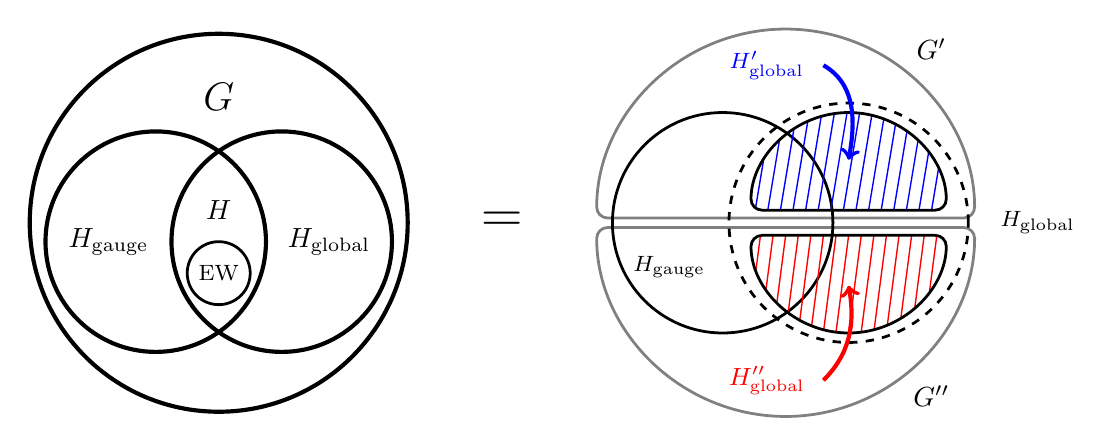
\begin{tikzpicture}[line width=1.5 pt, scale=.8]
%\draw (0,0) circle (3);

\begin{scope}[shift={(-9,0)}]
\draw (0,0) circle (3);
\draw (1,-.3) circle (1.75);
\draw (-1,-.3) circle (1.75);
\node at (0,2) {\Large $G$};
\node at (1.75,-.3) { $H_\text{global}$};
\node at (-1.75,-.3) { $H_\text{gauge}$};
%\node at (0,-.3) {\Large $H$};
\node at (0,.2) {$H$};
\draw[line width=1pt] (0,-.8) circle (.5);
\node at (0,-.8) {\footnotesize EW};
\end{scope}

\begin{scope}[shift={(-4.5,0)}]
\node at (0,0) {\huge =};
\end{scope}



\begin{scope}[shift={(0,0.075)}]
\draw[rounded corners, line width=1, color=gray] (3,0) arc (0:180:3) -- cycle;
\end{scope}

\begin{scope}[shift={(0,-0.075)}]
\draw[rounded corners, line width=1, color=gray] (-3,0) arc (180:360:3) -- cycle;
\end{scope}

\draw[line width=1] (-1,0) circle (1.75);
\draw[dashed, line width=1] (1,0) circle (1.9);

\begin{scope}[shift={(1.,0)}]
\begin{scope}[shift={(0,.2)}]%[rotate=0]% [rotate=-45]
    \begin{scope}
    	\clip [rounded corners] (1.55,0) arc (0:180:1.55) -- cycle;
    	\foreach \x in {-1.9,-1.7,...,1.3}
	    \draw[line width=.5 pt, color=blue] (\x,-1.3) -- (\x+.6,2.3);
    \end{scope}
    \draw[rounded corners, line width=1] (1.55,0) arc (0:180:1.55) -- cycle;
\end{scope}
\begin{scope}[shift={(0,-.2)}]%[rotate=0]%[rotate=45]
    \begin{scope}
    	\clip [rounded corners] (-1.55,0) arc (180:360:1.55) -- cycle;
    	\foreach \x in {-1.9,-1.7,...,1.3}
	    \draw[line width=.5 pt, color=red] (\x,-2.3) -- (\x+.6,2.3);
    \end{scope}
    \draw[rounded corners, line width=1] (-1.55,0) arc (180:360:1.55) -- cycle;
\end{scope}
\end{scope}
%\draw[line width=2pt] (0,-.4) circle (.4);
\node at (4,0) {\footnotesize $H_\text{global}$};
\node at (-1.85,-.7) {\footnotesize $H_\text{gauge}$};
\node at (50:3.6) {$G'$};
\node at (-50:3.6) {$G''$};
\path[->, color=blue, line width=1.5] (.6,2.5) edge [out = -30, in = 80] (1,1);
\node at (-.3,2.5) {\footnotesize \textcolor{blue}{$H_\text{global}'$}};
\path[->, color=red, line width=1.5] (.6,-2.5) edge [out = 45, in = 280] (1,-1);
\node at (-.3,-2.5) {\small \textcolor{red}{$H_\text{global}''$}};
\end{tikzpicture}
\end{center}





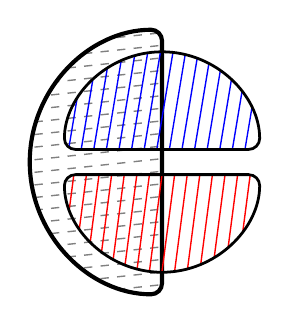
\begin{tikzpicture}[line width=1.5 pt, scale=.8]
%\draw (0,0) circle (3);



%\draw[line width=1] (-1,0) circle (1.75);
%\draw[dashed, line width=1] (0,0) circle (1.9);



\begin{scope}[rotate=90]
\begin{scope}
    	\clip [rounded corners] (2.1,0) arc (0:180:2.1) -- cycle;
    	\foreach \x in {-2.9,-2.7,...,3.3}
	    \draw[line width=.5 pt, color=gray, dashed] (\x,-2.3) -- (\x-.6,3.3);
    \end{scope}
    \draw[rounded corners, line width=1.5] (2.1,0) arc (0:180:2.1) -- cycle;
\end{scope}

\begin{scope}[shift={(0,.2)}]%[rotate=0]% [rotate=-45]
    \begin{scope}
    	\clip [rounded corners] (1.55,0) arc (0:180:1.55) -- cycle;
    	\foreach \x in {-1.9,-1.7,...,1.3}
	    \draw[line width=.5 pt, color=blue] (\x,-1.3) -- (\x+.6,2.3);
    \end{scope}
    \draw[rounded corners, line width=1] (1.55,0) arc (0:180:1.55) -- cycle;
\end{scope}
\begin{scope}[shift={(0,-.2)}]%[rotate=0]%[rotate=45]
    \begin{scope}
    	\clip [rounded corners] (-1.55,0) arc (180:360:1.55) -- cycle;
    	\foreach \x in {-1.9,-1.7,...,1.3}
	    \draw[line width=.5 pt, color=red] (\x,-2.3) -- (\x+.6,2.3);
    \end{scope}
    \draw[rounded corners, line width=1] (-1.55,0) arc (180:360:1.55) -- cycle;
\end{scope}

%\draw[line width=2pt] (0,-.4) circle (.4);
%\node at (4,0) {\footnotesize $H_\text{global}$};
%\node at (-1.85,-.7) {\footnotesize $H_\text{gauge}$};
%\node at (50:3.6) {$G'$};
%\node at (-50:3.6) {$G''$};
%\path[->, color=blue, line width=1.5] (.6,2.5) edge [out = -30, in = 80] (1,1);
%\node at (-.3,2.5) {\footnotesize \textcolor{blue}{$H_\text{global}'$}};
%\path[->, color=red, line width=1.5] (.6,-2.5) edge [out = 45, in = 280] (1,-1);
%\node at (-.3,-2.5) {\small \textcolor{red}{$H_\text{global}''$}};
\end{tikzpicture}
\qquad
\qquad
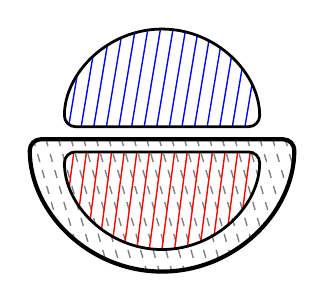
\begin{tikzpicture}[line width=1.5 pt, scale=.8]
%\draw (0,0) circle (3);



%\draw[line width=1] (-1,0) circle (1.75);
%\draw[dashed, line width=1] (0,0) circle (1.9);

\begin{scope}[rotate=180]
\begin{scope}
    	\clip [rounded corners] (2.1,0) arc (0:180:2.1) -- cycle;
    	\foreach \x in {-2.9,-2.7,...,3.3}
	    \draw[line width=.5 pt, color=gray, dashed] (\x,-2.3) -- (\x-1.6,3.3);
    \end{scope}
    \draw[rounded corners, line width=1.5] (2.1,0) arc (0:180:2.1) -- cycle;
\end{scope}

\begin{scope}[shift={(0,.2)}]%[rotate=0]% [rotate=-45]
    \begin{scope}
    	\clip [rounded corners] (1.55,0) arc (0:180:1.55) -- cycle;
    	\foreach \x in {-1.9,-1.7,...,1.3}
	    \draw[line width=.5 pt, color=blue] (\x,-1.3) -- (\x+.6,2.3);
    \end{scope}
    \draw[rounded corners, line width=1] (1.55,0) arc (0:180:1.55) -- cycle;
\end{scope}
\begin{scope}[shift={(0,-.2)}]%[rotate=0]%[rotate=45]
    \begin{scope}
    	\clip [rounded corners] (-1.55,0) arc (180:360:1.55) -- cycle;
    	\foreach \x in {-1.9,-1.7,...,1.3}
	    \draw[line width=.5 pt, color=red] (\x,-2.3) -- (\x+.6,2.3);
    \end{scope}
    \draw[rounded corners, line width=1] (-1.55,0) arc (180:360:1.55) -- cycle;
\end{scope}

%\draw[line width=2pt] (0,-.4) circle (.4);
%\node at (4,0) {\footnotesize $H_\text{global}$};
%\node at (-1.85,-.7) {\footnotesize $H_\text{gauge}$};
%\node at (50:3.6) {$G'$};
%\node at (-50:3.6) {$G''$};
%\path[->, color=blue, line width=1.5] (.6,2.5) edge [out = -30, in = 80] (1,1);
%\node at (-.3,2.5) {\footnotesize \textcolor{blue}{$H_\text{global}'$}};
%\path[->, color=red, line width=1.5] (.6,-2.5) edge [out = 45, in = 280] (1,-1);
%\node at (-.3,-2.5) {\small \textcolor{red}{$H_\text{global}''$}};
\end{tikzpicture}
\qquad
\qquad
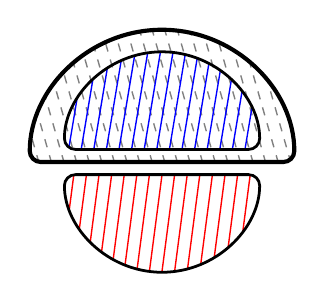
\begin{tikzpicture}[line width=1.5 pt, scale=.8]
%\draw (0,0) circle (3);



%\draw[line width=1] (-1,0) circle (1.75);
%\draw[dashed, line width=1] (0,0) circle (1.9);

\begin{scope}[rotate=0]
    \begin{scope}
    	\clip [rounded corners] (2.1,0) arc (0:180:2.1) -- cycle;
    	\foreach \x in {-2.9,-2.7,...,3.3}
	    \draw[line width=.5 pt, color=gray, dashed] (\x,-2.3) -- (\x-1.6,3.3);
    \end{scope}
    \draw[rounded corners, line width=1.5] (2.1,0) arc (0:180:2.1) -- cycle;
\end{scope}

\begin{scope}[shift={(0,.2)}]%[rotate=0]% [rotate=-45]
    \begin{scope}
    	\clip [rounded corners] (1.55,0) arc (0:180:1.55) -- cycle;
    	\foreach \x in {-1.9,-1.7,...,1.3}
	    \draw[line width=.5 pt, color=blue] (\x,-1.3) -- (\x+.6,2.3);
    \end{scope}
    \draw[rounded corners, line width=1] (1.55,0) arc (0:180:1.55) -- cycle;
\end{scope}
\begin{scope}[shift={(0,-.2)}]%[rotate=0]%[rotate=45]
    \begin{scope}
    	\clip [rounded corners] (-1.55,0) arc (180:360:1.55) -- cycle;
    	\foreach \x in {-1.9,-1.7,...,1.3}
	    \draw[line width=.5 pt, color=red] (\x,-2.3) -- (\x+.6,2.3);
    \end{scope}
    \draw[rounded corners, line width=1] (-1.55,0) arc (180:360:1.55) -- cycle;
\end{scope}

%\draw[line width=2pt] (0,-.4) circle (.4);
%\node at (4,0) {\footnotesize $H_\text{global}$};
%\node at (-1.85,-.7) {\footnotesize $H_\text{gauge}$};
%\node at (50:3.6) {$G'$};
%\node at (-50:3.6) {$G''$};
%\path[->, color=blue, line width=1.5] (.6,2.5) edge [out = -30, in = 80] (1,1);
%\node at (-.3,2.5) {\footnotesize \textcolor{blue}{$H_\text{global}'$}};
%\path[->, color=red, line width=1.5] (.6,-2.5) edge [out = 45, in = 280] (1,-1);
%\node at (-.3,-2.5) {\small \textcolor{red}{$H_\text{global}''$}};
\end{tikzpicture}










\section{Minimal Moose}

	\begin{tikzpicture}[line width=1.5]
	\begin{scope}
	    \begin{scope}
	    	\clip (-.5,0) circle (.5);
	    	\foreach \x in {-2.5,-2.4,...,.3}
				\draw[line width=.8 pt] (\x,-1.9) -- (\x+1.5,1);
	  	\end{scope}
    	\draw[line width = 1.5] (0,0) circle (1);
    	\draw[line width = 1.5] (-.5,0) circle (.5);
    	
    	\draw[line width = 1.5] (4,0) circle (1);
    	\begin{scope}
	    	\clip (4,0) circle (.8);
	    	\begin{scope}[shift={(4,0)}]
	    	\clip (0,0) circle (.8);
	    	\foreach \x in {-2.5,-2.4,...,.3}
				\draw[line width=.8 pt] (\x,-1.9) -- (\x+1.5,1);
	  	\end{scope}
	  	\end{scope}
    	\draw[line width = 1.5] (4,0) circle (.8);
    	
    	\draw[fermion] (1,0) -- (3,0);
    	\node at (-1.6,0) {$G_\text{EW}$};
    	\node at (0.1,1.4) {$\text{SU}(3)_\text L$};
    	\node at (4.1,1.4) {$\text{SU}(3)_\text R$};
    	\node at (5.9,0) {$\text{SU}(3)_\text R$};
    	\node at (2,.5) {$\Sigma$};
	\end{scope}
	\end{tikzpicture}
	
	
	\vspace{1em}
	
	\begin{tikzpicture}[line width=1.5]
	\begin{scope}
	    \begin{scope}
	    	\clip (-.5,0) circle (.5);
	    	\foreach \x in {-2.5,-2.4,...,.3}
				\draw[line width=.8 pt] (\x,-1.9) -- (\x+1.5,1);
	  	\end{scope}
    	\draw[line width = 1.5] (0,0) circle (1);
    	\draw[line width = 1.5] (-.5,0) circle (.5);
    	
    	\draw[line width = 1.5] (4,0) circle (1);
    	\begin{scope}
	    	\clip (4,0) circle (.8);
	    	\begin{scope}[shift={(4,0)}]
	    	\clip (0,0) circle (.8);
	    	\foreach \x in {-2.5,-2.4,...,.3}
				\draw[line width=.8 pt] (\x,-1.9) -- (\x+1.5,1);
	  	\end{scope}
	  	\end{scope}
    	\draw[line width = 1.5] (4,0) circle (.8);
    	
    	\draw[fermion] (1,0) -- (3,0);
	 \end{scope}
	\begin{scope}[shift={(0,-2.3)}]
	    \begin{scope}
	    	\clip (-.5,0) circle (.5);
	    	\foreach \x in {-2.5,-2.4,...,.3}
				\draw[line width=.8 pt] (\x,-1.9) -- (\x+1.5,1);
	  	\end{scope}
    	\draw[line width = 1.5] (0,0) circle (1);
    	\draw[line width = 1.5] (-.5,0) circle (.5);
    	
    	\draw[line width = 1.5] (4,0) circle (1);
    	\begin{scope}
	    	\clip (4,0) circle (.8);
	    	\begin{scope}[shift={(4,0)}]
	    	\clip (0,0) circle (.8);
	    	\foreach \x in {-2.5,-2.4,...,.3}
				\draw[line width=.8 pt] (\x,-1.9) -- (\x+1.5,1);
	  	\end{scope}
	  	\end{scope}
    	\draw[line width = 1.5] (4,0) circle (.8);
    	
    	\draw[fermion] (1,0) -- (3,0);
	 \end{scope}
	 \begin{scope}[shift={(0,-4.6)}]
	    \begin{scope}
	    	\clip (-.5,0) circle (.5);
	    	\foreach \x in {-2.5,-2.4,...,.3}
				\draw[line width=.8 pt] (\x,-1.9) -- (\x+1.5,1);
	  	\end{scope}
    	\draw[line width = 1.5] (0,0) circle (1);
    	\draw[line width = 1.5] (-.5,0) circle (.5);
    	
    	\draw[line width = 1.5] (4,0) circle (1);
    	\begin{scope}
	    	\clip (4,0) circle (.8);
	    	\begin{scope}[shift={(4,0)}]
	    	\clip (0,0) circle (.8);
	    	\foreach \x in {-2.5,-2.4,...,.3}
				\draw[line width=.8 pt] (\x,-1.9) -- (\x+1.5,1);
	  	\end{scope}
	  	\end{scope}
    	\draw[line width = 1.5] (4,0) circle (.8);
    	
    	\draw[fermion] (1,0) -- (3,0);
	 \end{scope}
	 \begin{scope}[shift={(0,-6.9)}]
	    \begin{scope}
	    	\clip (-.5,0) circle (.5);
	    	\foreach \x in {-2.5,-2.4,...,.3}
				\draw[line width=.8 pt] (\x,-1.9) -- (\x+1.5,1);
	  	\end{scope}
    	\draw[line width = 1.5] (0,0) circle (1);
    	\draw[line width = 1.5] (-.5,0) circle (.5);
    	
    	\draw[line width = 1.5] (4,0) circle (1);
    	\begin{scope}
	    	\clip (4,0) circle (.8);
	    	\begin{scope}[shift={(4,0)}]
	    	\clip (0,0) circle (.8);
	    	\foreach \x in {-2.5,-2.4,...,.3}
				\draw[line width=.8 pt] (\x,-1.9) -- (\x+1.5,1);
	  	\end{scope}
	  	\end{scope}
    	\draw[line width = 1.5] (4,0) circle (.8);
    	
    	\draw[fermion] (1,0) -- (3,0);
	 \end{scope}
	 \begin{scope}[shift={(-3.5, -3.45)}]
	     \begin{scope}
	    	\clip (0,0) circle (.5);
	    	\foreach \x in {-2.5,-2.4,...,.3}
				\draw[line width=.8 pt] (\x,-1.9) -- (\x+1.5,1);
	  	\end{scope}
	  	\draw[line width = 1.5] (0,0) circle (.5);
	  	\draw[dashed, line width=1.5, ->] (60:.75) -> (60:4);
	  	\draw[dashed, line width=1.5, ->] (-60:.75) -> (-60:4);
	  	\draw[dashed, line width=1.5, ->] (20:.75) -> (20:2.2);
	  	\draw[dashed, line width=1.5, ->] (-20:.75) -> (-20:2.2);
	 \end{scope}
    \begin{scope}[shift={(7.8, -3.45)}]
	     \begin{scope}
	    	\clip (0,0) circle (.8);
	    	\foreach \x in {-2.5,-2.4,...,.3}
				\draw[line width=.8 pt] (\x,-1.9) -- (\x+1.5,1);
	  	\end{scope}
	  	\draw[line width = 1.5] (0,0) circle (.8);
	  	\draw[dashed, line width=1.5, ->] (120:1.1) -> (120:4);
	  	\draw[dashed, line width=1.5, ->] (-120:1.1) -> (-120:4);
	  	\draw[dashed, line width=1.5, ->] (160:1.1) -> (160:2.2);
	  	\draw[dashed, line width=1.5, ->] (-160:1.1) -> (-160:2.2);
	 \end{scope}
	\node at (-4.8,-3.45) {$G_\text{EW}$};
	\node at (9.7,-3.45) {$\text{SU}(3)_\text{R}$};
    \end{tikzpicture}






\section{RS}


\begin{tikzpicture}[scale=.6,every node/.style={minimum size=1cm},on grid, rotate=0]
		
% Adapted from TikzExamples

    \begin{scope}[
            yshift=-83,every node/.append style={
            yslant=0.5,xslant=-1},yslant=0.5,xslant=-1
            ]
            
        %% BOTTOM LAYER
        % opacity to prevent graphical interference
        \fill[white,fill opacity=0.9] (0,0) rectangle (5,5);
        \begin{scope}[shift={(1.945,1.945)}]
            \draw[black, thick] (0,0) rectangle (1.111,1.111);
            \draw[step=.370333, gray] (0,0) grid (1.111,1.111);
        \end{scope}
        \draw[blue, dashed] (0,0) rectangle (5,5);%marking borders
    \end{scope}
    
    %% NEXT TO BOTTOM	
    \begin{scope}[
    	yshift=0,every node/.append style={
    	    yslant=0.5,xslant=-1},yslant=0.5,xslant=-1
    	             ]
        \fill[white,fill opacity=.8] (0,0) rectangle (5,5);
        \draw[blue,dashed] (0,0) rectangle (5,5);
        \begin{scope}[shift={(1.667,1.667)}]
            \draw[black, thick] (0,0) rectangle (1.666,1.666);
            \draw[step=.555333, gray] (0,0) grid (1.666,1.666);
        \end{scope}
    \end{scope}
    
    %% NEXT TO TOP
    \begin{scope}[
    	yshift=90,every node/.append style={
    	yslant=0.5,xslant=-1},yslant=0.5,xslant=-1
    	             ]
    	\fill[white,fill opacity=.7] (0,0) rectangle (5,5);
    	\begin{scope}[shift={(.84,.84)}]
    	    \draw[black, step=1.106] (0,0) grid (3.318,3.318);
        	\draw[black,very thick] (0,0) rectangle (3.318,3.318);
    	\end{scope}
    	\draw[blue,dashed] (0,0) rectangle (5,5);
    \end{scope}
    	
    	
    %% TOP
    \begin{scope}[
    	yshift=170,every node/.append style={
    	    yslant=0.5,xslant=-1},yslant=0.5,xslant=-1
    	  ]
        \fill[white,fill opacity=0.8] (0,0) rectangle (5,5);
        \draw[step=5/3, black] (0,0) grid (5,5);
        \draw[black, very thick] (0,0) rectangle (5,5);
    \end{scope}

    	
%  http://tex.stackexchange.com/questions/33607/easy-curves-in-tikz

%    \draw[fill=blue] (0,-1) circle (.08);
%    \draw[fill=blue] (-1.1,-.43) circle (.08);
%    \draw[fill=blue] (1.1,-.43) circle (.08);
%    \draw[fill=blue] (1.65,2.48) circle (.08);
%    \draw[fill=blue] (3.3,5.65) circle (.08);
%    \draw[fill=blue] (4.98,8.46) circle (.08);
%    \draw[fill=blue] (5.7,9) circle (.08);
    
    \node[name=a1] at (1.1,-.43) {};
    \node[name=a2] at (1.65,2.48) {};
    \node[name=a3] at (3.3,5.65) {};
    \node[name=a4] at (4.98,8.46) {};
    
    
    \node[name=b1] at (-1.1,-.43) {};
    \node[name=b2] at (-1.65,2.48) {};
    \node[name=b3] at (-3.3,5.65) {};
    \node[name=b4] at (-4.98,8.46) {};
    
    \draw [red, line width=2, opacity=.8] plot [smooth, tension=1] coordinates { (a1) (a2) (a3) (a4)};
    \draw [red, line width=2, opacity=.8] plot [smooth, tension=1] coordinates { (b1) (b2) (b3) (b4)};
    
    \draw [black, line width = 2,->] (-9, -1) -- (-9, 9.9);
    \node at (-9.5, 9) {\large $z$}; 
    \draw [black, line width = 2,->] (-8, 9.5) -- (-8, -1.5);
	 \node at (-7.5, -.5) {\large $\mu$}; 
	 
	 \node[rotate=90] at (-9.5, 4) {\large extra dimension};
	 \node[rotate=-90] at (-7.5, 5) {\large renormalization scale};
	
\end{tikzpicture}



\section*{Acknowledgements}


This work is supported in part by the \textsc{nsf} grant \textsc{phy}-1316792. 
%
%\textsc{p.t.}\ thanks 
%\emph{your name here}
%for useful comments and discussions. 

%% Appendices
% \appendix

% \bibliographystyle{utphys} 
% \bibliography{bib title without .bib}

\end{document}